\documentclass{standalone}
\usepackage{pgfplots}

\pgfplotsset{width=7cm,compat=newest}

\begin{document}

% ROUGE 1
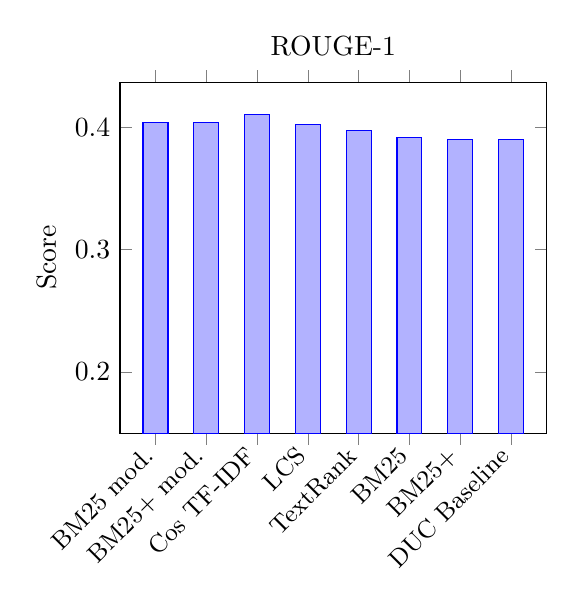
\begin{tikzpicture}
\begin{axis}[
title=ROUGE-1,
xtick={BM25 mod.,BM25+ mod.,Cos TF-IDF,LCS,TextRank,BM25,BM25+,DUC Baseline},
x tick label style={rotate=45,anchor=east,font=\small},
ylabel=Score,
symbolic x coords={BM25 mod.,BM25+ mod.,Cos TF-IDF,LCS,TextRank,BM25,BM25+,DUC Baseline},
ymin={0.150000},
ybar=5pt,
bar width=9pt
]
\addplot
coordinates {
        (BM25 mod.,0.4042)
        (BM25+ mod.,0.4040)
        (Cos TF-IDF,0.4108)
        (LCS,0.4020)
        (TextRank,0.3972)
        (BM25,0.3916)
        (BM25+,0.3903)
        (DUC Baseline,0.3900)
};
\end{axis}
\end{tikzpicture}


% ROUGE 2
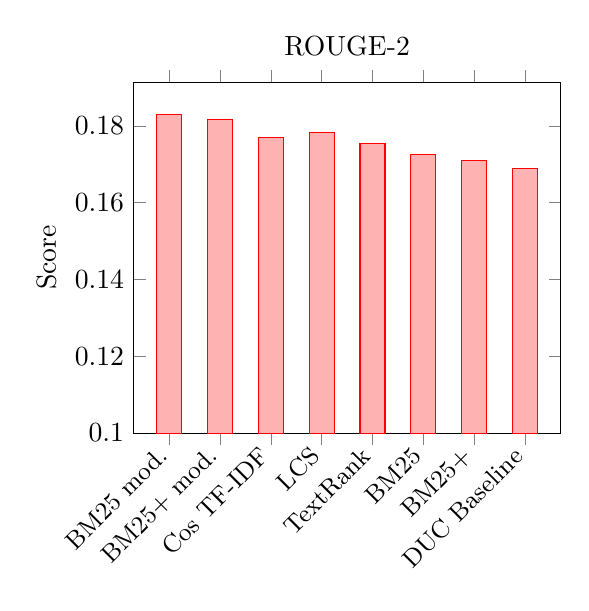
\begin{tikzpicture}
\begin{axis}[
title=ROUGE-2,
xtick={BM25 mod.,BM25+ mod.,Cos TF-IDF,LCS,TextRank,BM25,BM25+,DUC Baseline},
x tick label style={rotate=45,anchor=east,font=\small},
ylabel=Score,
symbolic x coords={BM25 mod.,BM25+ mod.,Cos TF-IDF,LCS,TextRank,BM25,BM25+,DUC Baseline},
ymin={0.10000},
ybar=5pt,
bar width=9pt
]
\addplot[red,fill=red!30]
coordinates {
        (BM25 mod.,0.1831)
        (BM25+ mod.,0.1818)
        (Cos TF-IDF,0.1770)
        (LCS,0.1783)
        (TextRank,0.1755)
        (BM25,0.1725)
        (BM25+,0.1711)
        (DUC Baseline,0.1689)
};
\end{axis}
\end{tikzpicture}

\end{document}
